% Copyright (c) 2017-2020 Matematyka dla Ciekawych Świata (http://ciekawi.icm.edu.pl/)
% Copyright (c) 2017-2020 Robert Ryszard Paciorek <rrp@opcode.eu.org>
% 
% MIT License
% 
% Permission is hereby granted, free of charge, to any person obtaining a copy
% of this software and associated documentation files (the "Software"), to deal
% in the Software without restriction, including without limitation the rights
% to use, copy, modify, merge, publish, distribute, sublicense, and/or sell
% copies of the Software, and to permit persons to whom the Software is
% furnished to do so, subject to the following conditions:
% 
% The above copyright notice and this permission notice shall be included in all
% copies or substantial portions of the Software.
% 
% THE SOFTWARE IS PROVIDED "AS IS", WITHOUT WARRANTY OF ANY KIND, EXPRESS OR
% IMPLIED, INCLUDING BUT NOT LIMITED TO THE WARRANTIES OF MERCHANTABILITY,
% FITNESS FOR A PARTICULAR PURPOSE AND NONINFRINGEMENT. IN NO EVENT SHALL THE
% AUTHORS OR COPYRIGHT HOLDERS BE LIABLE FOR ANY CLAIM, DAMAGES OR OTHER
% LIABILITY, WHETHER IN AN ACTION OF CONTRACT, TORT OR OTHERWISE, ARISING FROM,
% OUT OF OR IN CONNECTION WITH THE SOFTWARE OR THE USE OR OTHER DEALINGS IN THE
% SOFTWARE.

% BEGIN: ssh
\subsection{powłoka zdalna}
Komenda
\texttt{ssh [user@]host}
umożliwia uzyskanie powłoki zdalnego systemu poprzez szyfrowane połączenie, przydatne opcje:\\
	\texttt{-L portLokalny:hostZdalny:portZdalny} tworzy tunel przekierowujący dane kierowane na portLokalny komputera na którym działa klient ssh do portu portZdalny na serwerze hostZdalny poprzez serwer SSH (przydatne gdy hostZdalny jest osiągalny z hostSSH ale nie z komputera lokalnego)\\
	\texttt{-D port} tworzy tunel dynamiczny na wskazanym porcie (może on być użyty jako proxy typu SOCKS np. w Firefoxie w celu zapewnienia dostępu do zasobów WWW dostępnych z serwera SSH a niedostępny z komputera lokalnego)\\
	\texttt{-p port} określa inny niż domyślny port serwera SSH\\
	\texttt{-X} aktywuje przekazywanie komend X serwera ze strony zdalnej do klienta (pozwala na uruchomienie po stronie zdalnej aplikacji z GUI, które zostanie wyświetlone na lokalnym X serwerze)

\begin{center}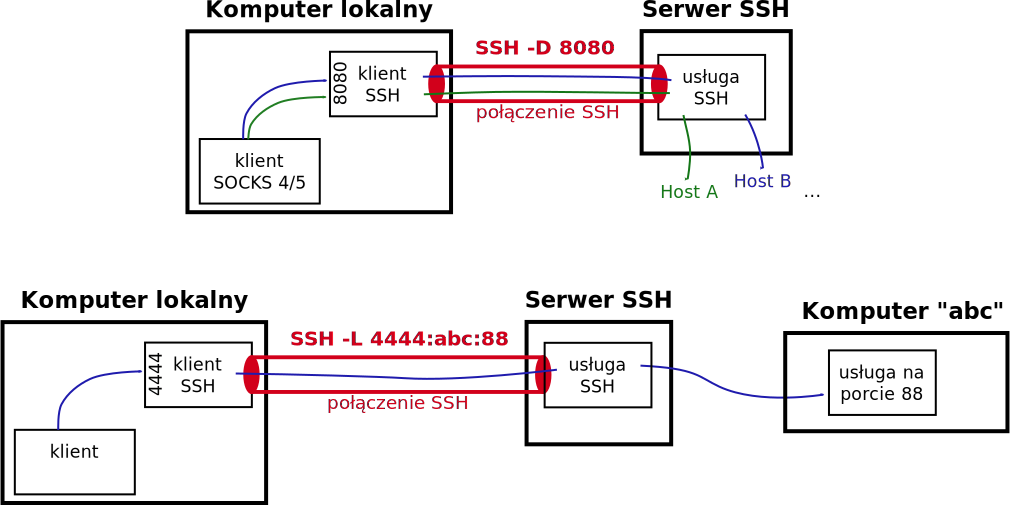
\includegraphics[width=0.7\textwidth]{img/linux/tunele_ssh}\end{center}
% END: ssh
